\begin{figure}
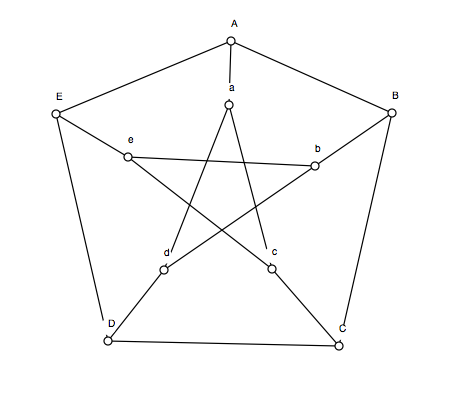
\includegraphics[scale=.5]{petersengraph}
\caption{Petersen Graph}
\end{figure}
As can be seen on the Petersen Graph above
by performing contractions on edges $aA, bB, cC, dD, eE$ we get a graph 
isomorphic to $K_5$. Since the Petersen  Graph contains a contraction of $K_5$ 
by Kuratowski's theorem the Petersen graph is not planar.
\begin{figure}
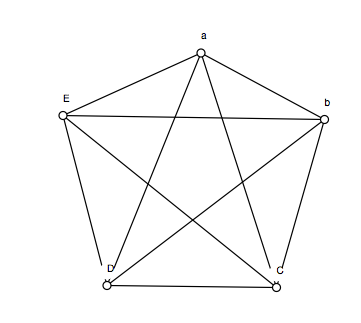
\includegraphics[scale=.5]{k5}
\caption{Contraction of Petersen Graph}
\end{figure}
